\documentclass[a4paper,12pt]{article}

\usepackage[top = 2.5cm, bottom = 2.5cm, left = 2.5cm, right = 2.5cm]{geometry}
\usepackage[T1]{fontenc}
\usepackage[utf8]{inputenc}
\usepackage{hyperref}
\usepackage{multirow}
\usepackage{booktabs,amsmath,amsthm}
\usepackage{changepage}
\usepackage{graphicx} 
\usepackage{setspace}
\usepackage{amsthm}
\usepackage{comment}
\usepackage{float}
\usepackage{fancyhdr}
\usepackage{pgfplots}

\setlength{\parindent}{0in}
\pagestyle{fancy} 
\fancyhf{}
\pgfplotsset{compat=1.18}

\newtheoremstyle{nonitalic}
  {3pt}
  {3pt}
  {\normalfont}
  {}
  {\bfseries}
  {.}
  {.5em}
  {}

\theoremstyle{nonitalic}

\newtheorem{definition}{Definition}[subsection]

\newtheorem{theorem}{Theorem}[subsection]

\lhead{\footnotesize STA260 Notes}
\rhead{\footnotesize sytez} 
\cfoot{\footnotesize \thepage}

\begin{document}
    \thispagestyle{empty}

    \begin{tabular}{p{15.5cm}}  
        {\Large \bf STA260 Notes}\\
        By sytez\\
        \hline
    \end{tabular}

    \begin{center}
        {\Large \bf Preface}
    \end{center}

    \quad These notes were made for the course STA260: Probability and Statistics II at the University of Toronto Mississauga. They are based on the lectures and lecture slides of the 2024 summer offering. This course was instructed by Professor Luai Al Labadi (The Goat). These notes primarily consist of a summary of the defintions and theorems from the course. The notes are not exhaustive and may contain errors. The proofs provided are not complete and instead provide a brief outline of the proof containing the main ideas. Theorems that do not contain a proof are usually trivial to prove with exceptions of the ones whose proof is beyond the scope of this course.

    \newpage
    
    \tableofcontents
    \newpage

    \setcounter{section}{6}

    \section{Chapter 7 \textemdash{} Sampling Distributions and the Central Limit Theorem}

    \subsection{Introduction}

    \begin{definition}
        A \textbf{population} consists of the entire collection of the observations with which we are concerned.
    \end{definition}

    \begin{definition}
        A \textbf{sample} is a subset of a population.
    \end{definition}

    \begin{definition}
        A \textbf{parameter} is a numerical summary of a population. For example, the mean, the variance, etc. In practice, it is unknown.
    \end{definition}

    \begin{definition}
        A \textbf{statistic} is a numerical summary of a sample. For example, the sample mean, the sample variance, etc.
    \end{definition}

    \begin{definition}
        The statistic varies from sample to sample and hence it is a random variable and has a probability distribution called the \textbf{sampling distribution}.
    \end{definition}

    The knowledge of the sampling distribution of a statistic helps to make an inference about the corresponding population (true) parameter.

    \begin{definition}
        We say that the random variables $Y_1, Y_2, \ldots, Y_n$ are \textbf{independent and identically distributed} (i.i.d.) if they are independent random variables and have the same probability distribution (same pdf/cdf).
    \end{definition}

    For a random sample, we write
    \[
        Y_1, \ldots, Y_n \overset{\text{i.i.d.}}{\sim} f(y) \quad \text{(continuous)}
    \]
    \[
        Y_1, \ldots, Y_n \overset{\text{i.i.d.}}{\sim} p(y) \quad \text{(discrete)}
    \]
    \newpage

    \subsection{Sampling Distributions}
    
    \begin{definition}
        The \textbf{sample mean} is defined as
        \[
            \overline{Y} = \frac{1}{n} \sum_{i=1}^{n} Y_i
        \]
    \end{definition}

    \begin{definition}
        The \textbf{sample variance} is defined as
        \[
            S^2 = \frac{1}{n-1} \sum_{i=1}^{n} (Y_i - \overline{Y})^2
        \]
    \end{definition}

    \begin{theorem}
        If $Y_1, \ldots, Y_n \overset{\text{i.i.d.}}{\sim} N\left(\mu, \sigma^2\right)$, then
        \[
        \overline{Y} \sim N\left(\mu, \frac{\sigma^2}{n}\right)
        \]
    \end{theorem}
    
    
    \begin{proof}
        Show MGF of $\overline{Y}$ is the MGF of $N\left(\mu, \frac{\sigma^2}{n}\right)$ then conclude by uniqueness of MGF.
    \end{proof}
    
    \begin{definition}
        The \textbf{standard normal distribution} is defined as
        \[
            Z = \frac{Y - \mu}{\sigma} = \frac{\overline{Y} - \mu}{\sigma/\sqrt{n}} = N(0,1)
        \]
    \end{definition}

    \begin{theorem}
        Let \( Y_1, \ldots, Y_n \overset{\text{i.i.d.}}{\sim} N(\mu, \sigma^2) \). If \( Z_i = \frac{Y_i - \mu}{\sigma} \), then
        \[
        \sum_{i=1}^{n} Z_i^2 = \sum_{i=1}^{n} \left( \frac{Y_i - \mu}{\sigma} \right)^2
        \]
        has a \(\chi^2\) distribution with \(n\) degrees of freedom (df)
    \end{theorem}
    
    \begin{proof}
        Note 3 facts:
        \begin{enumerate}
            \item \(\chi^2_{(v)} = \text{Gamma}(v/2, 2)\)
            \item \(\chi^2_{(v_1)} + \chi^2_{(v_2)} \sim \chi^2_{(v_1 + v_2)}\) assuming independence
            \item \([N(0,1)]^2 = Z^2 \sim \chi^2_{(1)}\)
        \end{enumerate}

        The proof becomes trivial from here.
    \end{proof}

    Note that similarly we have the sum of many distributions can be studied easily.
    \[\begin{aligned}
        &Y_1, \ldots, Y_n \overset{\text{iid}}{\sim} \text{Ber}(p) \implies \sum_{i=1}^{n} Y_i \sim \text{Bin}(n, p) \\
        &Y_1, \ldots, Y_n \overset{\text{iid}}{\sim} \text{Poisson}(\lambda) \implies \sum_{i=1}^{n} Y_i \sim \text{Poisson}(n\lambda) \\
        &Y_1, \ldots, Y_n \overset{\text{iid}}{\sim} \chi^2(v_i) \implies \sum_{i=1}^{n} Y_i \sim \chi^2_{\left(\sum\limits_{i=1}^{n} v_i\right)}\\
        &Y_1, \ldots, Y_n \overset{\text{iid}}{\sim} N(\mu_i, \sigma^2_i) \implies \sum_{i=1}^{n} Y_i \sim N\left(\sum\limits_{i=1}^{n} \mu_i, \sum\limits_{i=1}^{n} \sigma^2_i\right)
    \end{aligned}\]

    \begin{proof}
        Note the following fact:\\
        Let $U = Y_1 + \ldots + Y_n$ then we have $M_U(t) = M_{Y_1}(t) \cdot \ldots \cdot M_{Y_n}(t)$.\\
        That is that the MGF of the sum of random variables is the product of the MGFs of the random variables.\\
        The proof follows trivially using the unqiueness of MGFs.
    \end{proof}

    \begin{theorem}
        As a corollary of theorem 1.2.2\\
        If \( Y_1, \ldots, Y_n \overset{\text{i.i.d.}}{\sim} N(\mu, \sigma^2) \), then
        \[
            U = \sum_{i=1}^{n} \left( \frac{Y_i - \mu}{\sigma} \right)^2 \sim \chi^2_{(n)}
        \]
        similarly one sees that if \( Y_i \sim N(\mu_i, \sigma_i^2), \, i = 1, \ldots, n \) (and independent), then
        \[
        U = \sum_{i=1}^{n} \left( \frac{Y_i - \mu_i}{\sigma_i} \right)^2 \sim \chi^2(n).
        \]
    \end{theorem}

    \begin{theorem}
        Let \( Y_1, Y_2, \ldots, Y_n \) be a random sample from a normal distribution with mean \(\mu\) and variance \(\sigma^2\). Then
        \[
        \frac{(n-1)S^2}{\sigma^2} = \sum_{i=1}^{n} \frac{(Y_i - \overline{Y})^2}{\sigma^2} \sim \chi^2_{n-1}.
        \]
        Additionally, \(\overline{Y}\) and \(S^2\) are independent.
    \end{theorem}

    \newpage

    \subsection{The t-Distribution}

    \begin{definition}
        Let $Z \sim N(0,1)$ and $W \sim \chi^2_{(v)}$. Then if $Z$ and $W$ are independent then we say
        \[
            T = \frac{Z}{\sqrt{W/v}} \sim t_{(v)}
        \]
        has a \textbf{$t$-Distribution} with $v$ degrees of freedom.
    \end{definition}

    So far it was assumed that the population standard deviation $\sigma$ is known. However, this assumption may be unreasonable. We want to estimate both $\mu$ and $\sigma$. A natural statistic to deal with inferences on $\mu$ is
    \[
        T = \frac{\overline{Y} - \mu}{S/\sqrt{n}} \sim t_{(n-1)}
    \]
    
    \textbf{Properties of the $t$-Distribution}
    
    \begin{figure}[h!]
        \centering
        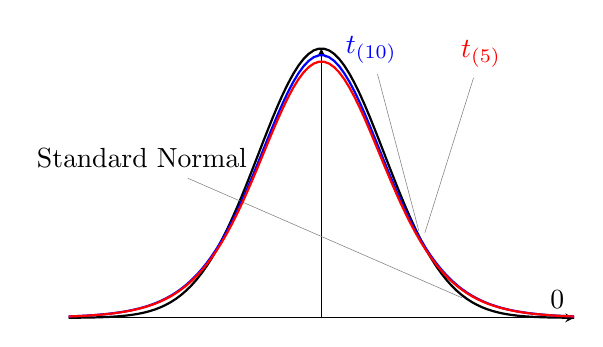
\begin{tikzpicture}
            \begin{axis}[
                axis lines=middle,
                xlabel={$0$},
                ylabel={},
                xtick=\empty,
                ytick=\empty,
                ymin=0,
                xmin=-4, xmax=4,
                samples=100,
                height=5cm,
                width=8cm,
                enlarge x limits=false,
                enlarge y limits=false,
                clip=false,
                ]
                % Standard Normal Curve
                \addplot[thick, black, domain=-4:4] {1/sqrt(2*pi) * exp(-0.5*x^2)} node[pos=0.8, pin={[pin distance=3cm]150:Standard Normal}] {};
                % t-distribution Curve (with 10 degrees of freedom)
                % (gamma(11/2)/(sqrt(10*pi)*gamma(5))) = 0.389108383
                \addplot[thick, blue, domain=-4:4] {0.389108383 * (1 + x^2/10)^(-11/2)} node[pos=0.7, pin={[pin distance=2cm]95:$t_{(10)}$}] {};
                % t-distribution Curve (with 5 degrees of freedom)
                % (gamma(3)/(sqrt(5*pi)*gamma(5/2))) = 0.379606689
                \addplot[thick, red, domain=-4:4] {0.379606689 * (1 + x^2/10)^(-11/2)} node[pos=0.7, pin={[pin distance=2cm]80:$t_{(5)}$}] {};
            \end{axis}
        \end{tikzpicture}
        \caption{Comparison of Standard Normal and $t$-distribution curves with 5 and 10 degrees of freedom}
    \end{figure}

    \begin{itemize}
        \item Each $t_\nu$ curve is bell-shaped and centered at 0.
        \item Each $t_\nu$ curve is spread out more than the standard normal ($Z$) curve.
        \item As $\nu$ increases, the spread of the corresponding $t_\nu$ curve decreases.
        \item As $\nu \to \infty$, the sequence of $t_\nu$ curves approaches the standard normal curve (the $Z$ curve is called a $t$ curve with df $=\infty$).
    \end{itemize}

    \newpage

    \subsection{The F-Distribution}

    \begin{definition}
        Let \( W_1 \sim \chi^2_{(\nu_1)} \) and \( W_2 \sim \chi^2_{(\nu_2)} \) be independent. Then
        \[
            F = \frac{W_1 / \nu_1}{W_2 / \nu_2}
        \]
        has a \textbf{\( F \)-Distribution} with \( \nu_1 \) and \( \nu_2 \) degrees of freedom.
    \end{definition}

    \begin{theorem}
        If \( S_1^2 \) and \( S_2^2 \) are the variances of independent random samples of size \( n_1 \) and \( n_2 \) taken from normal populations with variances \( \sigma_1^2 \) and \( \sigma_2^2 \), respectively, then
        \[
        \frac{S_1^2 / \sigma_1^2}{S_2^2 / \sigma_2^2} \sim F(n_1 - 1, n_2 - 1).
        \]        
    \end{theorem}

    \begin{proof}
        Recall that
        \[
            \frac{(n-1)S^2}{\sigma^2} \sim \chi^2_{(n-1)}
        \]
        the proof trivially follows.
    \end{proof}
    
    \begin{theorem}
        Let $Y$ be a random variable such that $Y \sim F_{(v_1, v_2)}$. Then
        \[
            \frac{1}{Y} \sim F_{(v_2, v_1)}
        \]
    \end{theorem}

    \begin{theorem}
        Let $Y_1 \sim F_{(v_1, v_2)}$ then
        \[
            \left(1 + \frac{v_1}{v_2}Y_1\right)^{-1} \sim \text{Beta}\left(\frac{v_2}{2}, \frac{v_1}{2}\right)
        \]
    \end{theorem}
    
    \begin{proof}
        Recall that
        \[
            \chi^2_{(v)} = \text{Gamma}\left(\frac{v}{2}, 2\right) \quad \text{and} \quad \frac{\text{Gamma}(\alpha, \gamma)}{\text{Gamma}(\alpha, \gamma) + \text{Gamma}(\beta, \gamma)} = \text{Beta}(\alpha, \beta)
        \]
        the proof follows trivially using the defintion of the $F$-distribution.
    \end{proof}

    \begin{theorem}
        Let $T$ be a random variable with a $t$-distribution with $v$ degrees of freedom. Then $U = T^2$ has an $F$-distribution with $1$ and $v$ degrees of freedom.
    \end{theorem}

    \newpage

    \subsection{The Central Limit Theorem}

    
\end{document}